\section{Application}

To empirically validate the feasibility of our proposed methodology, we developed a prototype application. This application contains it's frontend and backend. Users can use our frontend via web application that communicates with our backend that provides the assistant services. \\

TODO: Brief chapter description \\

\subsection{Assistant services}

Our LLM based assistant provides the following main services: (1) elements suggestion, (2) highlighting already modeled elements and (3) domain model summary.

\subsection{Elements suggestion}

TODO: Uvést obrázky podobně, jako to je v článku \\

When a domain description is provided the assistant generates suggestions solely based on the provided text. Otherwise, the assistant generates most relevant suggestions solely based on it's trained parameters.

Our assistant is able to suggest classes. For a selected class the assistant provides functionality to suggest it's attributes and associations. For a selected source class and selected target class the assistant is able to suggest their associations.


\subsubsection{Context highlighting}

As mentioned in the section (TODO: add section reference), for each suggested attribute and association we highlight it's context in the domain description. Additionally, for each class we highlight it's name. \\

TODO: info o tom, jakým způsobem se zotavujeme z chyb (například rozdíl mezi britskou a americkou angličtinou -- motorised vs. motorized) \\


\subsubsection{Elements conversion}
As an attribute can be usually modeled as an association and vice versa, for each attribute suggestion we provide functionality to convert any attribute to an association and vice versa. We convert an attribute into an association by putting the attribute name into the association target class. The opposite conversion works the same but in reverse.


\subsubsection{Duplicate elements}
The generated element suggestion is not shown to the user if he already modeled the corresponding element. We remove these suggestions on the backend after the LLM generates the output so we do not have to change the prompts. The element suggestion is removed if it's name syntactically matches the name of the user's corresponding modeled element. This approach has some limits such as semantically same elements but with a different name are not  removed. Possible solutions are to either use a LLM or some BERT based model as in retrieval-augmented generation however, both have significant disadvantages.

Solving the mentioned problem with a LLM in a single prompt approach complicates the prompt wording and can reduce the output quality. Using LLM in an iterative prompt approach can significantly increase the delay between the user's request and the suggestions displaying as the LLM has to process more than one prompt which can take many seconds.

When using some BERT based model as mentioned in the section (TODO: section reference), one of the challenging tasks is to set the decision boundary between accepting and rejecting the corresponding element. For example attributes ``first name'' and ``last name'' are very close in terms of vector space distance however, they represent a two distinct attributes. This fact would force us to set very strict decision boundary that would reject almost any two syntactically different words which is in result almost identical to our naive approach.


\subsubsection{Single field suggestion}

For the best possible output quality and response time when generating suggestions we try to simplify the prompt as much as possible. This for example means that the generated attributes suggestions does not contain their description or data type. For generating these additional fields we allow the user to edit any suggestions and use the LLM to suggest any of the given single field. \\

TODO: zmínit nastavení formátu pro jména až to budu mít naimplementované \\


\subsection{Highlighting already modeled elements}

We extend the mentioned highlighting of elements in the domain description by highlighting all the user's modeled elements in the domain description. \\

TODO: na jaké hlavní problémy jsem narazil a proč některé zvýrazněné prvky v popisu domény ve skutečnosti nemusí být namodelovány a naopak viz poznámky \\


\subsection{Summary of domain model}

For a selected part of the user's conceptual model the assistant is able to generate a summary for each class, attribute and association. We implemented two summary variations: in a plain text and in form of bullet points.

In both variations the corresponding prompt does not contain the user's domain description because we found out that our used LLM does not stick to the selected conceptual model when it gets both the user's conceptual model and the domain description as the input.

The plain text summary generates a paragraph describing the user's selected domain model. We let the user to set the style of this summary. The available styles are ``analytical'', ``educational'' and ``funny story''. When a style is selected the prompt for plain text summary is edited so it instructs the LLM to generate the output in the selected style.

The summary in form of bullet points for each element generates a description. In the future by adding options to accept, reject or regenerated each description this could be used to help the user to create a description for each of his modeled element for a better domain model documentation.


\subsection{LLM parameters}

TODO: možná by se tato sekce více hodila jinam \\

TODO: co je to temperature a proč ji nastavujeme na 0 \\

TODO: možná zmínit problém se snahou vygenerovat pokaždé jiný výstup \\


\subsection{LLM output parsing}

TODO: zmínit hlavní věci, které se dějí při parsování výstupu + odkázat se na to, že odstraňování duplicitních elementů jsme již pokryli v předchozí subsekci \\


\subsection{Saving user data}

For each generated suggestion the user can optionally click on the like button or the dislike dislike button. The corresponding evaluated suggestion is sent to the backend and saved there with all the parameters that were used to generate this suggestion. To remember these parameters, the frontend remembers for each suggestion the parameters that were used for generation.

We use these user's reactions for two main reasons. First reason is that we can use these data as a feedback. For example, we can automatically detect if some set of parameters repeatedly ended up with too many negative reactions. After that we can analyse the issue and fix it. Second reason is that we can use these data to fine-tuning some LLM to further improve the quality for our specific tasks.

The downside of our approach is that it does not collect many user data. One possible solution is to save each user action such as saving each suggestion that the user added into his domain model. However, this approach has a lot of disadvantages due to it's complexity. For example, if the user adds some suggestion and then later on removes it we need to save this removal action too as it can mean that the original suggestion turned out to be unwanted. This means that the saved data would need to be post-processed to remove these pairs of data. Similar issue arise when user adds some suggestion but then later on edits it. Because of this complexity we decided to use the explicit reactions buttons.


\subsection{Work-flow}

Figure \ref{fig:work-flow} shows the basic flow of generating suggestions on the backend. The modeling process typically starts by providing the domain description. Then the domain model is step by step created by using suggestions from the assistant. Suggestions of attributes and associations are filtered by some retrieval-augmentation method. Then the prompt engineering techniques are applied and the final prompt is constructed and sent to LLM. Finally, the output from the LLM is parsed and the suggested model elements are sent back to the frontend. \\

TODO: Asi popsat, že v nastavení si uživatel může vybrat variantu filtrování popisu domény \\

\begin{figure}[!h]
    \centering
    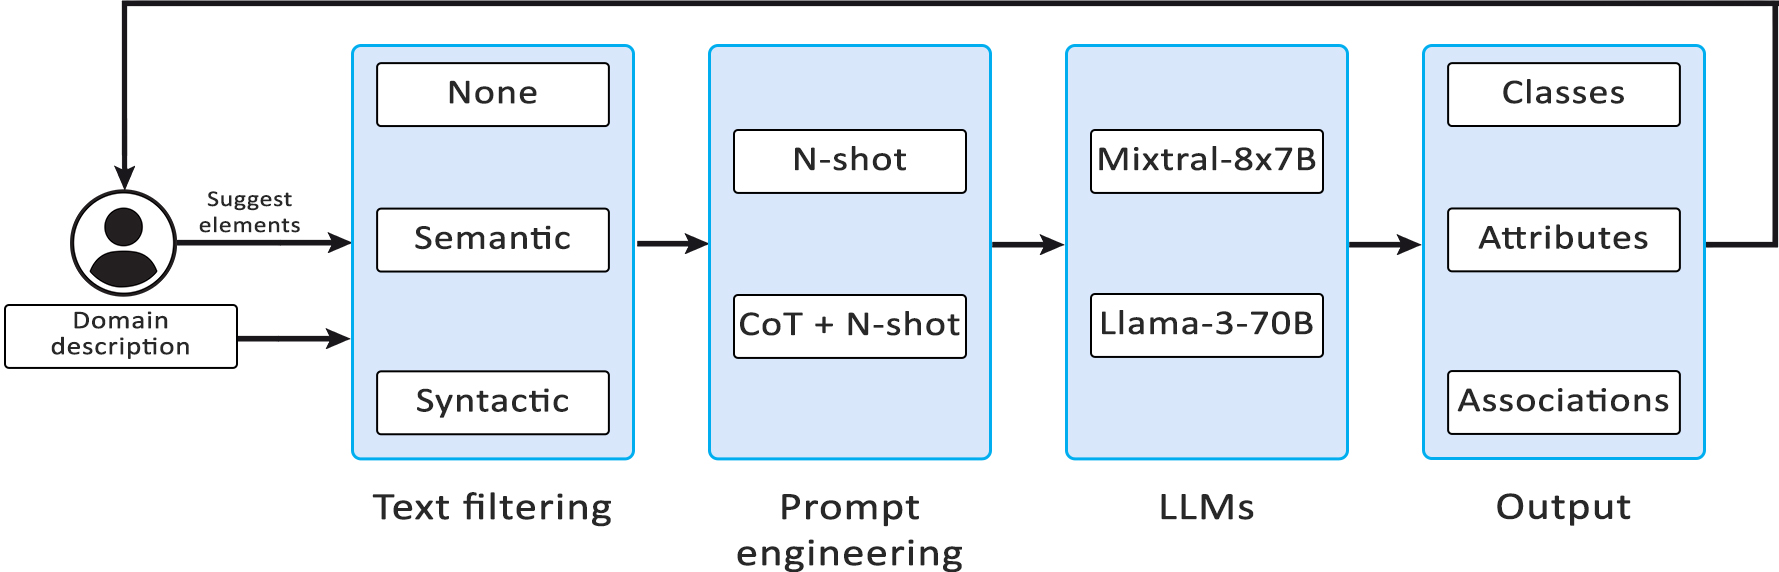
\includegraphics[scale=0.23]{img/work-flow.jpg}
    \caption{\centering Schema of the flow of processing the textual domain description}
    \label{fig:work-flow}
\end{figure}
